\documentclass[11pt, a4paper]{article}
\usepackage[a4paper, margin = 0.7in]{geometry}
\usepackage{graphicx}
\usepackage{amsmath}
\usepackage{listings}
\usepackage{url}

\title{Assignment 3: Fitting Data To Models} % Title

\author{Aman Kumar EE19B066} % Author name

\date{\today} % Date for the report
\begin{document}	
		
\maketitle % Insert the title, author and date
\section{Abstract}
This week's assignment is about fitting data to models.
The main content of the assignment is: 
\begin{itemize}
    \item Reading data from files and parsing them
    \item Analysing the data to extract information
    \item To study the effects of noise on the fitting process.
    \item To plot a number of different types of plots. 
\end{itemize}

\section{Importing the data from file}
On running the python code \textit{\path{generate_data.py}}, it creates a file \textit{\path{fitting.dat}}. This gives rise to the following plot of a function with added noises.

\begin{figure}[h]
   	\centering
   	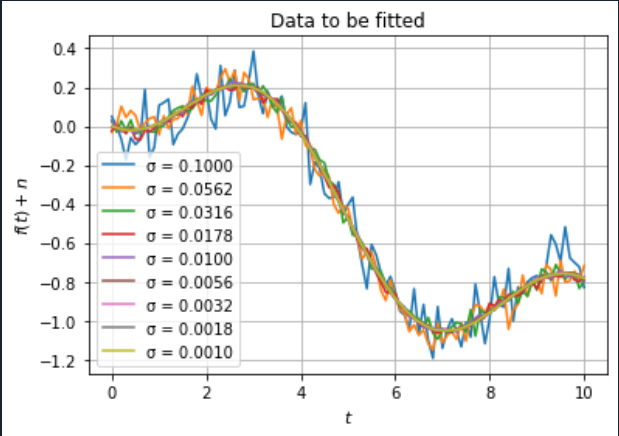
\includegraphics[scale=0.6]{Data to fit.png}   
   	\caption{Data to fit to assumed model}
   	\label{fig:Figure 0}
\end{figure} 
   This file contains 10 columns with 101 rows of data. The first column is time and the next nine columns are the values of the function with different amount of noise added. Each column of data has its own standard deviation which is given by the python command
\begin{verbatim}	
    stdev = logspace(-1,-3,9)
\end{verbatim}
To extract the data from the \textit{\path{fitting.dat}} file python's loadtxt function was used.
\begin{verbatim}
    data = np.loadtxt("fitting.dat")
    t = data[:,0]
\end{verbatim}
\section{The Function with Noisy plots}
Model function is given as:
\begin{verbatim}	
    def g(t,A,B):
        return(A*sp.jn(2,t) + B*t)
\end{verbatim}

Q3. and Q4. asks to plot the nine data columns along with the true value. The plot that is obtained is given below. The part of python code used for this:
\begin{verbatim}	
    for i in range(1,10):
        pl.plot(t,data[:,i],label="\u03C3 = %0.4f" % stdev[i-1])
    pl.plot(t,y0,label="True Value",color='black',linewidth = 3)	
\end{verbatim}
\begin{figure}[h]
   	\centering
   	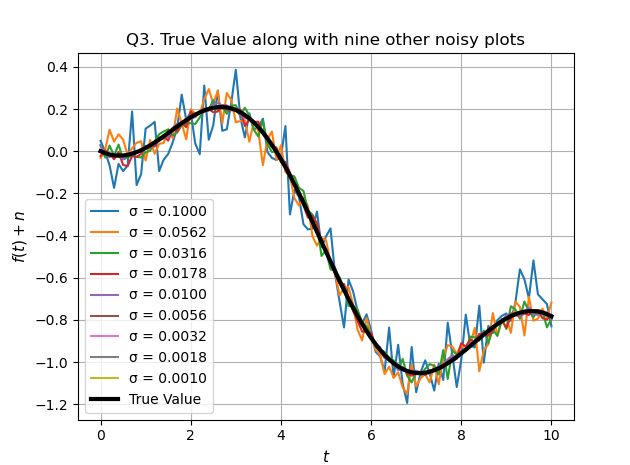
\includegraphics[scale=0.6]{Figure 0.png}   
   	\caption{True and noise added plots}
   	\label{fig:Figure 1}
\end{figure} 
   
\section{Plotting the Error Bars}
An errorbar is a convenient way of visualising the uncertainty in the reported measurement. The errorbars for the first data column are plotted using the \textbf{errorbar()} function. The part of python code used for plotting the errorbar plot::
\begin{verbatim}	
    pl.errorbar(t[::5],data[:,1][::5],stdev[1],fmt='ro',label="error bar")
    pl.plot(t,y0,label = "True value",color = 'black')
\end{verbatim}
 The graph obtained by plotting every 5th data point with errorbars and the original data is as follows:   
\begin{figure}[h]
   	\centering
   	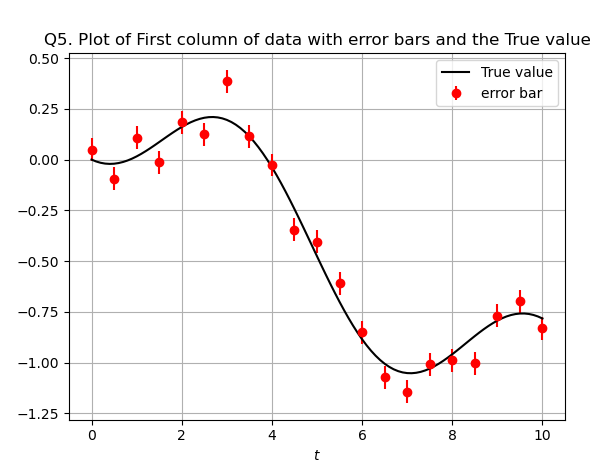
\includegraphics[scale=0.6]{ErrorBar.png}   
   	\caption{Errorbars with True value}
   	\label{fig:Figure 2}
\end{figure} 
See Figure \ref{fig:Figure 2} on page \pageref{fig:Figure 2}
  
\section{Generating the matrix}
The function can be created using a matrix equation also. The matrix M created when multiplied with (A,B) matrix will be equal to the value of function. This can be verified by substituting $A=1.05$ and $B=-0.105$. In order to compare 2 matrices, we use the function \path{array_equal()}. Python code:
\begin{verbatim}	
    Jt = sp.jn(2,t)
    M = pl.c_[Jt,t]
    if (np.array_equal(np.dot(M,A0B0),y0)):
        print("M*[A0;B0] is equal to g(t,A0,B0). Verified!")
    else:
        print("M*[A0;B0] is NOT equal to g(t,A0,B0).")
\end{verbatim} 
\section{Estimating A and B}
A and B are estimated by minimising the $\varepsilon_{ij}$. It is done here using \textbf{lstsq()} function as given below:
\begin{verbatim}
    def estimate_A_B(M,col):
        AB = pl.lstsq(M,col,rcond=None)
        return(AB[0][0],AB[0][1])
\end{verbatim}
\section{Mean Squared Error for Different A and B}
The mean squared error between the noisy data and the true value is calculated as follows:
$$\varepsilon_{ij} = (\frac{1}{101})\sum_{k=0}^{101}(f_{k} - g(t_{k},A_{i},B_{j}))^{2}$$
The python code to calculate the mean squared error is as follows:
\begin{verbatim}	
    A = np.linspace(0, 2, 21)
    B = np.linspace(-0.2, 0, 21)
    Err = np.zeros((21,21))
    f1 = data[:,1]
    for i in range(21):
        for j in range(21):
            Err[i,j] += np.sum(((f1 - g(t,A[i],B[j]))**2))/101
\end{verbatim}
The contour plot for $\varepsilon_{ij}$ for various values of A and B is:
\begin{figure}[!tbh]
   	\centering
   	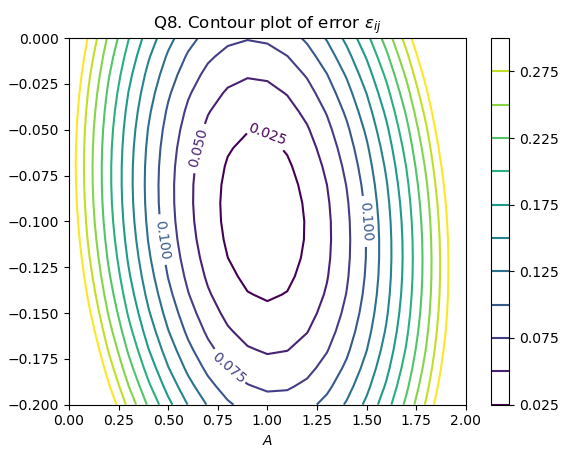
\includegraphics[scale=0.6]{Contour.png}   
   	\caption{Contour plot of $\varepsilon_{ij}$}
   	\label{fig:Figure 4}
\end{figure} 
     
\subsection{Conclusion}
From the above plot, we can conclude that there exist one and only one minimum for $\varepsilonepsilon_{ij}$ and as we move away from $A0,B0$ value of $\varepsilon_{ij}$ increases

\section{Error in the Estimation of A and B} 
$A,B$ are calculted by minimising $\varepsilon_{ij}$ by \textit{lstsq()} function form \textit{scipiy.linalg}. Since, we know $A0,B0$ we can calculate the MSerror in the values of A and B.Python code:
\begin{verbatim}	
    Aerr,Berr = np.zeros(9),np.zeros(9)
    for i in range(1,10):
        A_est,B_est = estimate_A_B(M,data[:,i])
        Aerr[i-1] += ((A_est - A0B0[0])**2)
        Berr[i-1] += (B_est - A0B0[1])**2
\end{verbatim}

The plot of the MSerror in A and B vs noise in linear and loglog scales:
\begin{figure}[!h]
   	\centering
   	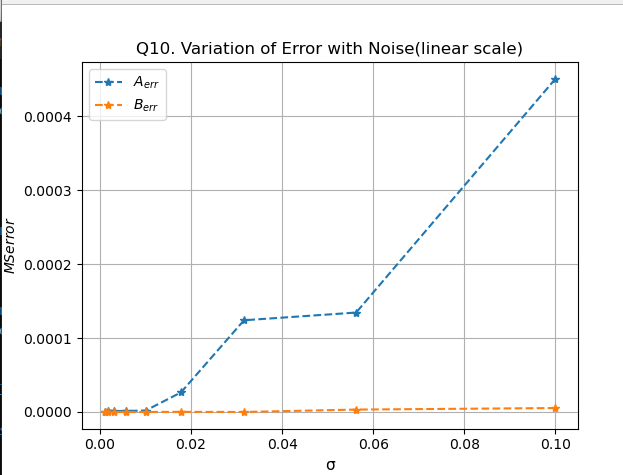
\includegraphics[scale=0.6]{Err with noise(linear).png}   
   	\caption{Error vs Standard deviation(linear scale)}
   	\label{fig:Figure 5}
\end{figure} 

\begin{figure}[!h]
   	\centering
   	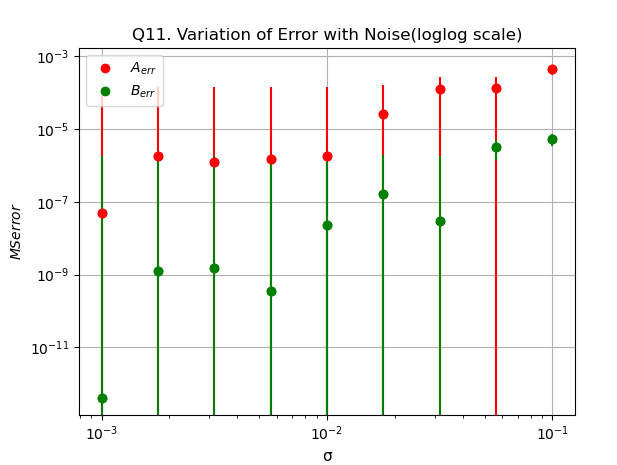
\includegraphics[scale=0.6]{Err with noise(loglog).png}   
   	\caption{Error vs Standard deviation(loglog)}
   	\label{fig:Figure 6}
\end{figure} 
The part of code used to plot the graph in Figure 5:
\begin{verbatim}
    pl.plot(stdev,Aerr,marker = "*",label="$A_{err}$",linestyle = 'dashed')
    pl.plot(stdev,Berr,marker = "*",label="$B_{err}$",linestyle = 'dashed')
\end{verbatim}
and Figure 6:
\begin{verbatim}
    pl.loglog(stdev,Aerr,'ro',label="$A_{err}$")
    pl.errorbar(stdev,Aerr,pl.std(Aerr),fmt='ro')
    pl.loglog(stdev,Berr,'go',label="$B_{err}$")
    pl.errorbar(stdev,Berr,pl.std(Berr),fmt='go')
\end{verbatim}

\subsection{Conclusion}
From figures 5 and 6 it is evident that the noise is linear in \textbf{neither} of the scales. This is because our noise varies on a logarithmic
scale and it is expected that the error must also vary in a logarithmic manner.

\section{Conclusion}
We have used the \textbf{lstsq()} function to fit a noisy data to a function. As the noise in the data used
to estimate the linear combination increases, the error in the estimation also
increases.
 
\end{document}
